\section{The Edenic State}

\paragraph{Magical Artist}

Suppose you saw a seascape that reminded you wistfully of that summer you spent in Cape Code in your youth … wouldn't you admire the artist? Now suppose there was a magical artist who, Escher-like, managed to paint you yourself into that seascape … how much more deeply would you re-experience that summer?

For the description of the primordial state, i.e., the state of man before the Fall, we are relying on the following two sources:

\begin{itemize}
\item \textbf{St Basil the Great}, \emph{On the Human Condition} 
\item \textbf{St Symeon the New Theologian}, \emph{The First Created Man} 
\end{itemize}
It is not enough to read it in an academic way, but rather one must try to ``enter the picture" and recognize their descriptions in one's own consciousness.

\paragraph{Executive Summary}
\begin{quotex}
The gnosis of the second Arcanum is consciousness such as it was before the Fall. \flright{\textsc{Valentin Tomberg}}

\end{quotex}
The Primordial state is the original state of human consciousness.

Man in the Primordial State is rational and passionless … this is the opposite of how man is viewed today. Of course, that is what we should expect, isn't it? The former describes man has he is in his essence, the latter, as he appears to be.

\begin{wrapfigure}{rt}{.3\textwidth}
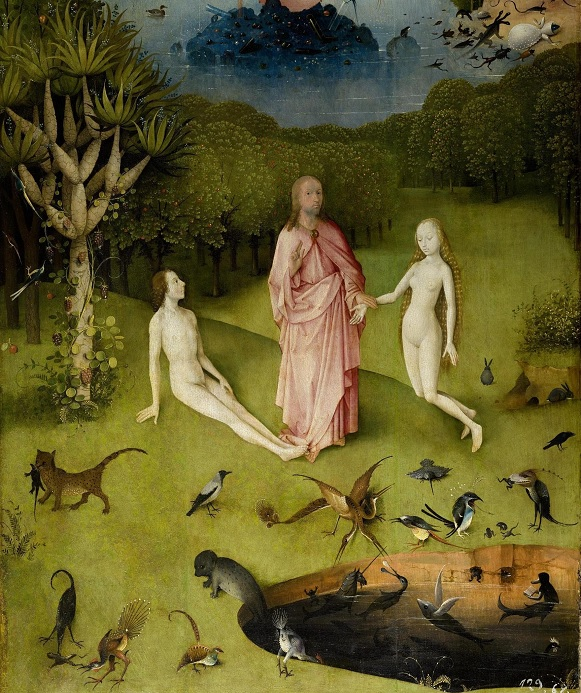
\includegraphics[scale=.3]{a20140926TheEdenicState-img001.jpg}
\caption{Earthly Delights}
\end{wrapfigure}

\paragraph{The Event Horizon}
Trying to understand the Genesis creation story historically and scientifically presents an immediate difficulty. Looking back in time, all we see is death and corruption. Any Edenic or primordial state is beyond that horizon and inaccessible to historical, archaeological, or scientific investigation. Nothing materially incorruptible could have survived until our time.

\paragraph{Psychic Layers}
In any case, it is not the historical events and conditions that counts, but rather their meaning. \textbf{Valentin Tomberg} develops a method of meditation which he attributes to \textbf{Carl Jung}. This involves ``the exploration of psychic layers as the living past of the soul. The entire past lives in the diverse layers of the depths of consciousness." So instead of looking back, we look inward to discover all the states of consciousness involved in the creation of the world and man.

God created the basic elements — light (fire), water, air, earth, and life — all of which are prerequisites for the possibility of manifestation. These elements symbolize energy and the three states of matter. Life signifies interiority, so that the world has an ``inside" as well as an ``outside". It is this interiority that makes such a meditation possible.

We have previously described this method to understand the cause of the Fall in \textit{Doubt and Certainty}\footnote{\url{https://www.meditationsonthetarot.com/doubt-and-certainty}}. With the help of the two Fathers who have described the primordial state in some detail, we offer suggestions to understand that state through the meditation of the psychic layers.

\paragraph{Image and Likeness}
Man was created in the image and likeness of God. These refer to the two poles of being, which is made clear because man is created both from spirit and dust:

\begin{itemize}
\item \textbf{Image of God}: This is man as created, so it is a passive quality. Just as a work of art brings glory to the artist, the image of God in man bears glory to God, not to man himself. This was not lost in the Fall. 
\item \textbf{Likeness to God}: The likeness to God occurs as man grows more god-like, which is called theosis. As an active quality, the likeness requires actualization and manifestation. This was lost in the Fall and its recovery is the goal of reintegration. 
\end{itemize}
Obviously, man as the image of God does not mean that God has a human type of body. Rather it means that man is distinguished by the rational, or intellectual, soul. Note especially that this does not mean that man \emph{has} reason, but rather that he \emph{is} reason. Man's body and lower soul is formed by the intellectual soul.

There is a lower and higher intellectual soul. The lower knows through discursive, logical, and sequential thought, the higher through direct intuition.

\begin{itemize}
\item \textbf{Lower intellect soul}: its function is to perceive the material world, then organize and evaluate these perceptions. 
\item \textbf{Higher intellect soul}: the higher function is to perceive spiritual realities. E.g. other people as spiritual beings, angels, and God 
\end{itemize}
These will be explained in detail in the forthcoming post on knowledge in Man, God, and Angels.

In the primordial state, the intellect works harmoniously with \emph{eros} (or \emph{epithumia}) and \emph{thumos}, the physical center and emotional center, respectively.

Thus man's real existence is interior: ``Although our outer human being is perishing, the inner is renewed day by day." [2 Cor 4:16]

\paragraph{New Age Distortions}
There are two new age distortions of this teaching, one for each pole. The first is the claim that everyone is a ``child of God" by birthright. The actual teaching is that only the baptized, i.e., those on the path to theosis, can be called children of God. The true meaning is that every human is created in the image of God, but that does not bring any glory or credit to that person.

The other is a corruption of the Vedanta idea that ``Atman is Brahman"; For example, people tell me, ``I am God," when I can see perfectly well that they are not. By that, they mean that in their fallen state they are somehow God-like. As we have seen, that is completely false. It is only by the reintegration to the Blessed State through theosis that makes someone ``God-like".

\paragraph{The Blessed State}
Since God is holy, passionless, and sinless, man in the blessed state is likewise holy, passionless, and sinless

\subparagraph{Holy}
The word for ``holy" in Greek and Hebrew means ``set apart", in English, it derives from ``whole". This refers to the Real I which is apart from and transcendent to the world. (``I am in the world but not of it.") The Real I also represents the unity of the being, since it ties all the parts together.

The holy man has no need of any law (with one exception), since a law commands us to do good and avoid evil. In Eden, all creation was good, hence there was no need to know evil.

\subparagraph{Changeable}
God is unalterable, unchangeable, and simple. Man, on the contrary, is alterable, changeable, and composed of parts. Although free from physical privation, there was still the possibility of mental privation. That is the meaning of the tree of good and evil. In other words, there was the possibility of knowing evil, but not the actuality. The Fall made that possibility actual as described in \textit{Doubt and Certainty}\footnote{\url{https://www.meditationsonthetarot.com/doubt-and-certainty}}.

Therefore, man as free was commanded not to eat from the tree lest he die. That was the only law.

\subparagraph{Sinless}
As created, the Will follows the Intellect. In the Primordial State, man was holy and he knew God directly through his intellect. As there were no distractions to the Will, it followed the Intellect faithfully. Hence, man was sinless.

This does not mean that man, such as he is, is sinless; that is the assumption of the modern mind. This usually is expressed that God created us a certain way, so our inclinations and peccadillos are how he wants us to be. Quite the contrary, we are to overcome such inclination and achieve the likeness of God through theosis.

There is a common misunderstanding about free will. The common opinion is that it means we can choose this or that at will. The deeper understanding of free will is that it means that we can never be compelled to choose evil. The practical application of this understanding is an exercise left to the reader.

\subparagraph{Passionless}
Passionless means that man in the primordial state was not subjected nor reactive to forces from below. It does not mean that he was cold and without feelings. After all, the world has an inside that can be felt deeply. Poets, artists, mystics, and even ordinary people have sometimes had this feeling of the world erupt into their consciousness. Although that feeling is quite profound, and even transforming, it is still natural and not the same as the unitive experience of theosis.

So passionless means that the Intellect rules over the passions; in particular, negative emotions cannot arise. Another way to put this is that the ``subtle rules the dense".

St Basil has an interesting interpretation of the command to ``rule" the animals. He allegorizes the animals as representing various emotional states, which must be ``ruled" by the Intellect.

The command to multiply means to increase our own spiritual growth.

\subparagraph{Conditions}
In the primordial state, man was immortal and incorrupt. There was no sin, sorrows, cares, or difficult necessities; there were no labors, no misfortunes, no disease, and no accidents.

These are the conditions that the New Age teachings assume as natural. The New Ager will assert that all is perfect, whole, and complete. Christian Science, in particular, claims to be based on the knowledge of those conditions.

However, those conditions only apply to man in the Primordial State. All affirmations, denials, treatments, visualizations, and so on are ineffective otherwise. A fortiori, all social programs to recreate the Edenic conditions are similarly doomed to failure. The modern mind rejects everything necessary for reintegration. They assume that:

\begin{itemize}
\item Man is not holy, but rather a part of nature. 
\item Man is not ruled by the Intellect, but rather by passions. These must be protected at all costs. Without passion, man is nothing. 
\item Man is not sinful, so whatever he is or does needs to be tolerated and accepted. 
\end{itemize}
Reintegration is based on the opposite of each of those assumptions.



\flrightit{Posted on 2014-09-26 by Cologero }

\begin{center}* * *\end{center}

\begin{footnotesize}\begin{sffamily}



\texttt{Marcel K. on 2014-09-26 at 13:31 said: }

Cologero,

I am a silent reader and since this is my first comment I want to thank you for the great work you've done with this blog and the profound insights you've given to us.

Since it is something I currently struggle to understand, I wanted to ask you if you could expand on the distinction between the state of passionlessness and the absence of feelings (or coldness)? I think you're telling us that it is possible to quench our passions without practicing a form of religious quietism, i.e. the complete suppression of our worldy efforts. Personally however I haven't been able to achieve a deep understanding of this distinction. It seems to me that whenever I think I begin to understand, it immediately slips from my grasp and I revert to a state of not-understanding. 

I've been wondering whether the distinction is blatantly obvious and my inability to comprehend simply a result of faulty thinking on my part, or very subtle with deeper implications than unsubtle distinctions.


\hfill

\texttt{Logres on 2014-09-26 at 22:08 said: }

If man is a microcosm, then the individual becomes just like Nature as we see it: that is, there is a blind, groping manifestation of undulating movement (which we mistakenly call ``real life" and identify our personality with), and then there is what the Catholics would call the ``hidden soul", which is what's left of the image of God in man. Just as the natural world undulates or groans for redemption, but by itself cannot manifest the Logos, so the fallen being is gripped by a fierce passion(s) which smothers up the waters of Life. Whoever wins at ``real life" loses, says Mouravieff, whoever ``loses", wins. The analogy, he states, is almost exact. Isn't this what is meant, the ``last will be first, the first last"? So the emotional (thumos) level of being is the aim of esoteric work, as it is embryonic, the astral foetus, and like embryonic tissue, is easily distorted by the power of the passions' toxins it is exposed to, in that under-developed state. That's why the personality has to ``die" in the dark night of the soul…it seems like cutting yourself off from Life, like an addiction. In reality, it's the way out that is ``deeper in".


\hfill

\texttt{Cologero on 2014-09-27 at 21:22 said: }

Marcel, that is a life's work, not a comment. Passionlessness means that one is not ruled by the lower passions. On the other hand, there are legitimate feelings that motivate our wills or else we'd be machines. I guess there is a subtle difference between the passions ruling or motivating. When the negative emotions are ignored, there is the possibility for higher feelings of joy, peace, etc. to appear. It requires study, e.g., in the Philokalia or Clement of Alexandria. And along with that, a lot of practice in observing the passions and learning not to be reactive.


\hfill

\texttt{Caleb on 2014-09-28 at 16:07 said: }

Marcel, 

It may help in understanding passionless to contemplate Aristotle's `Unmoved Mover.' Consider the relation of the Sun to the other heavenly bodies which orbit it. Its position relative to them remains unmoved, and yet even though it just sits there in the center, its mere presence determines the movement of the other celestial bodies through its gravis. One certainly would not describe the Sun as cold however! 

Passion can be defined as ``that which moves us." The sun, through its immense presence is not moved by the other bodies, which by traditional understanding represent the passions (Venus driving desire, Mars driving anger, the moon driving the subconscious, etc). God likewise is as the sun, the center and source of all things, which move in Him, while He, in His aspect of transcendent unity, remains unmoved, because He is the center. That is the ideal which we aim for as we make our way back to the center.


\hfill


\end{sffamily}\end{footnotesize}
